\section{Measuring the performance of the pipeline}\label{e2e}

Above results reflect the performance of the \ac{ASR} stage alone, (that is: the performance of the \ac{STT} engine). To get some insight about the quality of alignments produced by the whole pipeline, a simple web application was implemented that highlights the aligned parts of the transcript as the audio file is being played. This is very useful for an informal review, because the perceived quality of the alignments can be examined interactively. However, this method is not very systematic and unpractical for larger amounts of test data. To get a clearer sense of how well the pipeline performs, steps were taken to run large numbers of previously unseen samples of audio/text data through the pipeline and measure the quality of the final product (the alignments). This section describes how this was done.

\subsection{The quality of alignments}

Assessing the quality of alignments is not trivial because there is often no reference alignment to compare to. Even if there is one, assessing the quality of an alignment is somewhat subjective because a different alignment does not necessarily need to be worse (or better). Hence objectively quantifying the quality of the result of the pipeline is difficult because there is a a massive number of theoretically possible alignments for each audio/text combination. We can however derive a few objective criteria that make up good alignments:

\begin{enumerate}
	\item The aligned partial transcripts should not overlap each other because one audio segment can only map to exactly one portion of the transcript.
	\item The alignments should neither start nor end within word boundaries because that would be considered bad segmentation.
	\item The aligned partial transcripts should cover as much of the original transcript as possible (if the transcript contains no extra text like footnotes or annotations, which are usually not read out loud).
	\item The aligned partial transcripts should be at the correct position, (i.e. they should cover the actually spoken text) because that relates to the perceived quality of the result.
\end{enumerate}

The first criterion is enforced by changing the type of algorithm used for sequence alignment from a local to a global alignment algorithm. The \textit{Smith-Waterman} algorithm was used for the \ac{SA} stage in the IP8 project, which finds a local optimum for each transcript in isolation. The \ac{SA} stage in this project uses global sequence alignment (\textit{Needle-Wunsch} algorithm), which finds an optimal alignment for all partial transcrips at once.

The second criterion is ensured by adjusting some of the alignments so that they fall exactly on word boundaries. This is done by moving the alignment boundaries produced by the \textit{Needle-Wunsch} algorithm to the left or right, depending on which one is closer. 

The remaining two criteria can be quantified with the metrics shown in table \ref{alignment_quality} (note the corellation\footnote{positive correlation: higher is better, negative correlation: lower is better}).

\begin{table}[!htbp]
	\centering
	\begin{tabular}{llll}
		\toprule
		\thead{criterion} & \thead{metric} & \thead{correlation} \\
		\midrule
		3 & \makecell[l]{length of text in ground truth that is not aligned\\vs. total length of the ground truth} & negative\\ \\ 	
		4 & \makecell[l]{average \textit{Levensthein Similarity} between the transcript\\and the text in the ground truth corresponding to its alignment} & positive \\ 
		\bottomrule
	\end{tabular}
	\caption{Metrics to evaluate the quality of alignments}
	\label{alignment_quality}
\end{table}

Because the first metric measures how much of the target transcript is covered by the alignments, it is similar to the Recall ($R$) usually used for classification tasks, which measures how much of the target class was correctly classified. The second metric uses the \textit{Levenshtein Similarity}, which is calculated from the normalized \textit{Levensthein Distance} (edit distance, \ac{LER}):

\[ 
levenshtein\_simliarity(a,b) = 1 - \frac{ed(a,b)}{max(|a|, |b|, 1))}
\]

The \textit{Levenshtein Similarity} measures how well the inferences match up with the aligned part of the transcript and is therefore similar to Precision ($P$) used in classification, which measures the accuracy of the classified results. Figure \ref{precision_recall_fscore} visualize how the average Precision and Recall are calculated for both the alignments produced by the pipeline using the reference model and the alignments produced by the pipeline using the simplified model.

\begin{figure}[h!]
	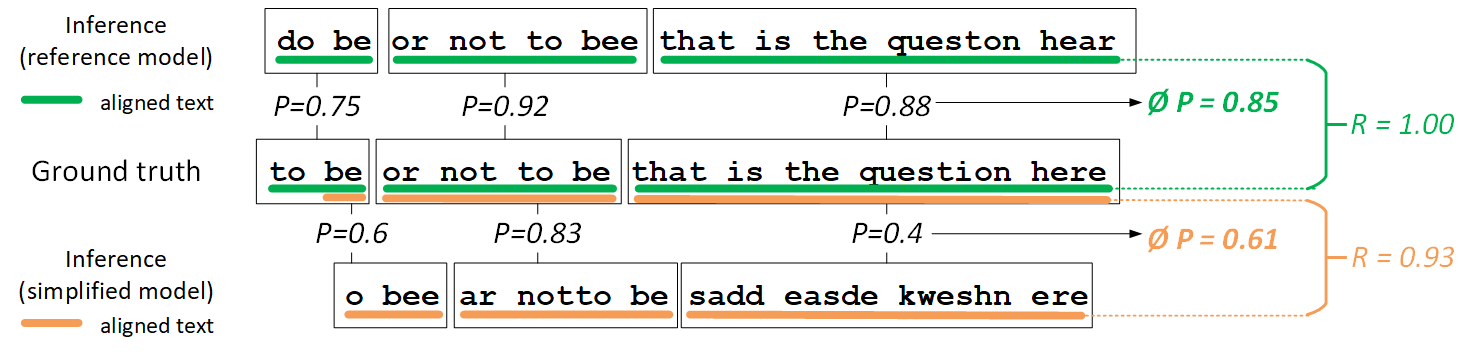
\includegraphics[width=\linewidth]{./img/precision_recall_fscore.png}
	\caption{Example of how Precision ($P$) and Recall ($R$) are calculated for alignments produced by the pipeline using the reference model and the alignments produced by pipeline using the simplified model.}
	\label{precision_recall_fscore}
\end{figure}

Both metrics can hence be reduced to the \textit{F-score} ($F$):

\[ 
F = 2\cdot \frac{P\cdot R}{P+R}
\]

All three metrics ($P$, $R$ and $F$) can be used to assess the quality of the result of a pipeline in isolation. To compare the quality of the alignments produced by the pipeline using the simplified model against a reference alignment however, it is compared against the results produced by the same pipeline using the \textit{DeepSpeech} model. The latter is considered a hypothetical optimal alignment. The comparison is made by calculating the \textit{Levensthein Distance} of the aligned texts, i.e. measuring how similar the alignments are. Figure \ref{alignment_similarity} illustrates how this is done for the alignments shown above.

\begin{figure}[h!]
	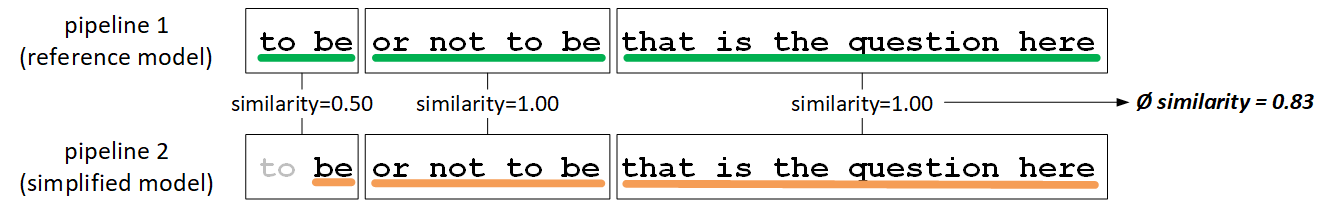
\includegraphics[width=\linewidth]{./img/alignment_similarity.png}
	\caption{Example of how the similarity between the alignments produced by the pipeline using the simplified model is compared to the alignments produced by the pipeline using the reference model (\textit{DeepSpeech}) for the alignments from Figure \ref{precision_recall_fscore}}
	\label{alignment_similarity}
\end{figure}


\subsection{Test and results}

The pipeline was evaluated on the test set of the \textit{LibriSpeech} corpus containing 87 audio/text samples (total audio length: 21:56:21). Each sample was run through the pipeline twice, once using the simplified model and once using the pre-trained \textit{DeepSpeech} model (reference model) in its \ac{ASR} stage. Apart from the model used in the \ac{ASR} stage, all other stages in the pipeline were identical, i.e. the audio was split into voiced segments only once. For the simplified model, the dropout-regularized variant of the simplified architecture was used and trained on $1,000$ minutes of training data because this combination had the lowest average \ac{LER} on the validation data. Training was stopped early after 15 epochs to prevent overfitting. Figure \ref{pipeline_boxplot_ls_en} shows for each model how the pipeline performs. 

\begin{figure}[h!]
	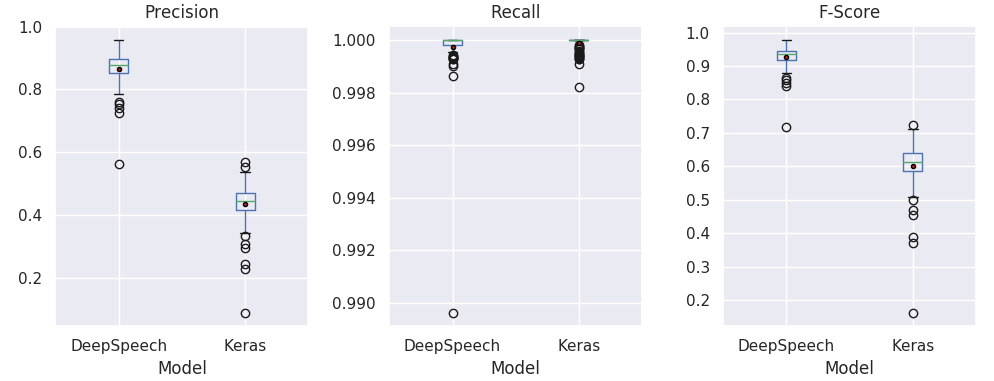
\includegraphics[width=\linewidth]{./img/boxplot_ls.png}
	\caption{Average values of $P$, $R$ and $F$ for a pipeline using the simplified \ac{STT} model compared to a pipeline using a state-of-the-art model. The box represents the range where 50\% of the data points are (\ac{IQR}). The whiskers extend to the last datum less than resp. greater than $1.5 \cdot IQR$. Data beyond the whiskers are outliers (marked as circles). The \textit{DeepSpeech} model produces very accurate transcripts and therefore very precise alignments ($P$ mean: $0.865$, median: $0.879$) and also a very high $F$-Score (mean: $0.926$, median: $0.935$). On the other hand, the simplified model produces only low-quality transcripts, resulting in a lower Precision (mean: $0.435$, median: $0.443$). The $F$-Score is thus also lower (mean: $0.602$, median: $0.614$). Recall is very high for both pipeline variants.}
	\label{pipeline_boxplot_ls_en}
\end{figure}

Obviously the \textit{DeepSpeech} model provides very accurate transcripts which makes alignment easy in the following \textit{\ac{GSA}} stage. Most values for $P$ lie therefore within a range of about $0.8$ and nearly $1.0$, except for a few outliers. The mean value is $0.865$. Because the simplified model was not trained for maximum speech recognition capabilities, the $P$-values are naturally lower and lie in a range of about $0.35$ and $0.55$ with a mean value of $0.435$. This is more or less consistent with the average normalized \ac{LER} on the validation set of about $0.52$.

In terms of coverage, both pipelines perform similarly well yielding mean $R$-values of $>0.999$. This is no surprise, because each alignment ends where the next one starts, thus there are no gaps and unaligned parts can only occur at the very start or end of a transcript. 

The $F$-score for the pipeline using the \textit{DeepSpeech} model is quite compact with most values lying in the interval $[0.875, 0.975]$ (mean value: $0.926$), whereas the range is a bit bigger for the pipeline using the simplified model (mean value: $0.602$).

When testing the alignments with the web application, the perceived quality is very good for both pipeline variants. Only in a few cases a word should be assigned to a different alignment.

Figure \ref{pipeline_scatterplot_ls_en} shows how the pipeline using the simplified model holds up against the pipeline using the reference model. It is evident that the \ac{LER} values between transcript and alignment are very low when using the reference model (left plot). When using the simplified model, the distribution of \ac{LER} values follows a similar pattern but is maybe a bit less compact on the y-axis and has a few more outliers. The mean average \ac{LER} value is $0.230$ when using the reference model and $0.982$ when using the simplified model. The length of the transcript resp. the recording does not seem to affect the performance of the alignment stage. Both pipeline variants can handle samples of various lenghts equally well. They both have however one striking outlier belonging to a very long transcript ($>15.000$ characters), which was read by a fast-speaking woman. 

\begin{figure}[h!]
	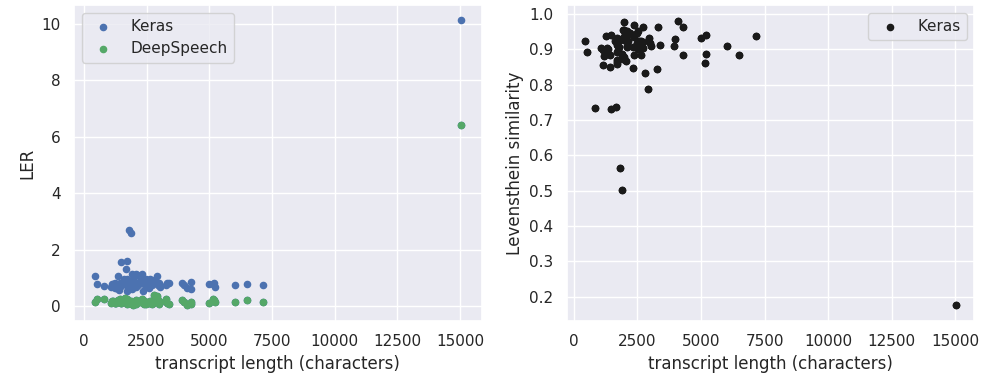
\includegraphics[width=\linewidth]{./img/scatterplot_ls.png}
	\caption{average \ac{LER} between transcript and alignment (left plot) and similarity between alignments produced by a pipeline using the reference model resp. the simplified model (right plot). The Average \ac{LER} values when using the simplified model (mean: $0.982$, median: $0.800$) follow the same pattern like when using the reference model (mean: $0.230$, median: $0.148$), but are generally higher due to the lower quality of the transcripts. However, this does not seem to affect the alignments produced by the two pipelines. The average similarity between alignments produced by the pipeline using the simplified model are roughly the same like when using the reference model (mean: $0.887$, median: $0.909$).}
	\label{pipeline_scatterplot_ls_en}
\end{figure}

When comparing the similarity between the alignments made using the reference model and those made using the simplified model (right plot) it is evident that the \textit{Levenshtein Similarity} is very high with a mean value of $0.887$, regardless of the transcript length. This means the alignments are almost identical, only differring in single words sometimes at beginnings/endings of alignments being assigned to the previous/next alignment. There are a few cases where the similarity is lower (and the long transcript mentioned before, where the alignments are not similar at all). However it can be generally said that despite the simplified model producing low-quality transcripts, the alignments do not differ much from the ones produced by a high-quality \ac{STT} engine.

\subsection{Summary}

This chapter demonstrated how the quality of alignments produced by the pipeline was measured. Since this quality is subjective, the results of the pipeline using the simplified \ac{STT} model were compared to the results of the same pipeline using the pre-trained \textit{DeepSpeech} model as a reference model. It was observed that although the quality of transcripts is notably lower for the former pipeline, the resulting alignments are very similar for both pipelines. This means the \ac{GSA} stage can handle transcripts of much lower quality and still produce good alignments.